\documentclass[10pt]{article}
\usepackage[margin=2.2cm]{geometry}
\usepackage{graphicx}\usepackage{booktabs}\usepackage{amsmath}\usepackage{amssymb}
\usepackage{xcolor}\usepackage[hidelinks]{hyperref}
\setlength{\parskip}{4pt}\setlength{\parindent}{0pt}
\graphicspath{{../../../output/05_pulsed_pupils/}}
\title{\vspace{-1.2cm}\textbf{Review 05 --- Pulsed $\times$ annular (new science)}\\
\large \texttt{mcdo\_dev} Phase 5 \quad(\texttt{output/05\_pulsed\_pupils/},
\texttt{docs/theory/05\_pulsed\_pupils.md})}
\author{}\date{2026-06-13}
\begin{document}\maketitle\vspace{-1.1cm}

\section*{The progress report's ``immediate next step''}
Eq.-10 spectral sum (full spectrum, Phase 1) over annular fields (Babinet,
Phase 3). $X_{NA}=0.8$, $\lambda_c$=750 nm, linear-$x$ y-cut, N\_freq=201.

\textbf{(i) Annular DOF extension is immune to few-cycle bandwidth.}
\begin{center}\small
\begin{tabular}{lcccc}
\toprule
DOF($\varepsilon$)/DOF(0) & cw & 5 fs & 2 fs & 1 fs\\\midrule
$\varepsilon=0.50$ & 1.30 & 1.30 & 1.30 & 1.30\\
$\varepsilon=0.90$ & 4.76 & 4.76 & 4.76 & 4.76\\
$\varepsilon=0.99$ & 44.35 & 44.35 & 44.34 & 44.33\\
\bottomrule
\end{tabular}
\end{center}
Invariant to 3 digits down to 1 fs (geometric $1/(1-\varepsilon^2)$, NA fixed
across frequencies). Each configuration's own DOF lengthens only $\sim$1.0\%
cw$\to$1 fs.

\textbf{(ii) Transverse ring contrast erodes with pulsing}, as the Romallosa
zeros did: Linfoot $S(1\,\text{fs})\to1.058$ across $\varepsilon$. Cross-check:
$\varepsilon=0$ gives $S(1\,\text{fs})=1.056$, matching Phase-1 single-photon
(1.053--1.062) --- pipeline confirmed.

\textbf{Flag:} $S(\tau)$ is \emph{non-monotonic} at high $\varepsilon$
($0.988\to0.987\to1.058$ for 5/2/1 fs) --- moderate pulses wash out the Bessel
rings ($S<1$) before 1-fs central broadening dominates ($S>1$). Plausible
ring-physics; $S(\text{cw,cw}){=}1$ and the $\varepsilon{=}0$ cross-check argue
against a bug; worth a dedicated ring-energy-vs-$\tau$ look if load-bearing.

\begin{center}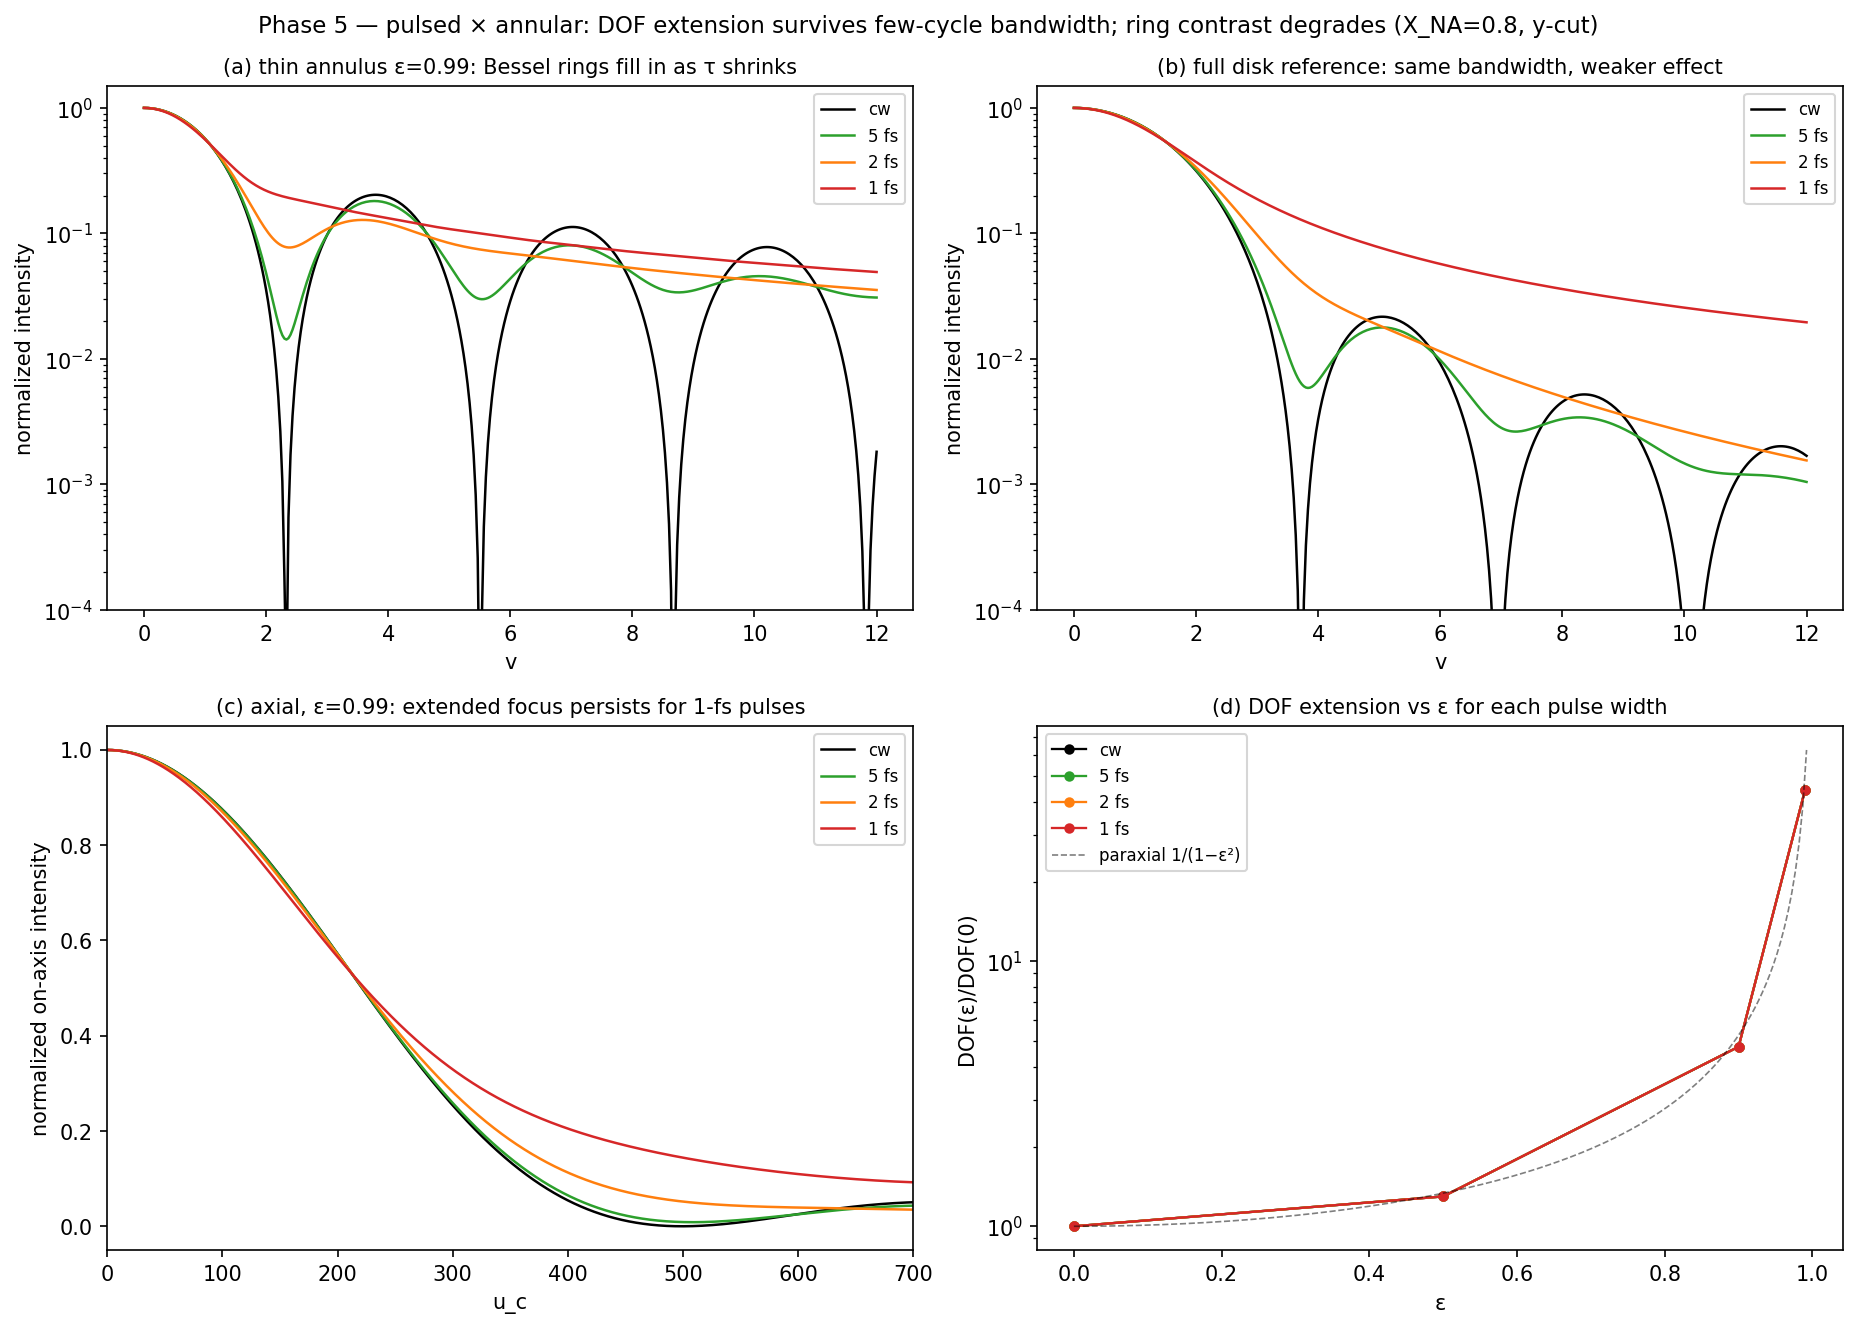
\includegraphics[width=0.99\textwidth]{verify_pulsed_annular.png}\end{center}
\textbf{(a)} $\varepsilon$=0.99 rings fill as $\tau\downarrow$; \textbf{(b)} full
disk reference; \textbf{(c)} axial extended focus persists at 1 fs;
\textbf{(d)} DOF($\varepsilon$)/DOF(0) curves for all $\tau$ overlie the
paraxial law.

\begin{center}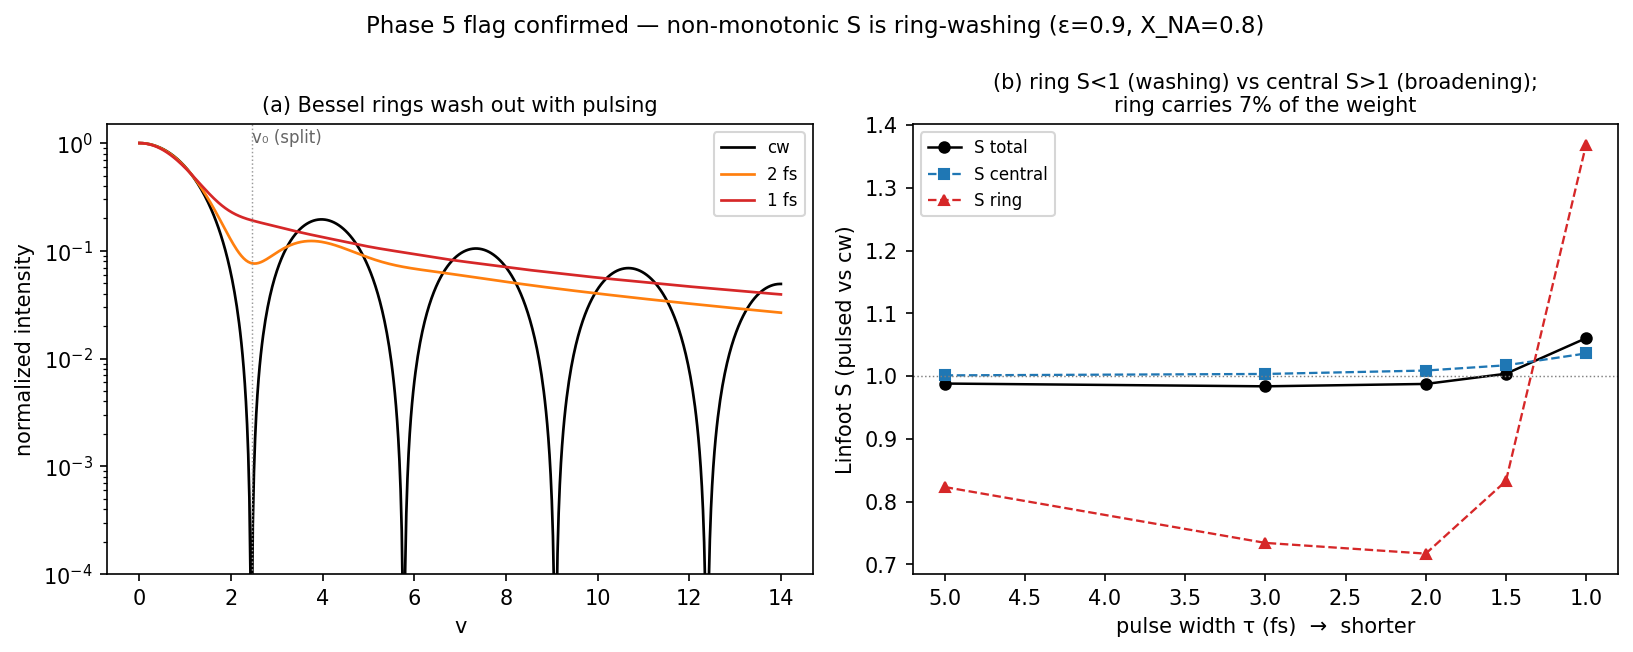
\includegraphics[width=0.95\textwidth]{ring_decomposition.png}\end{center}
\textbf{Flag confirmed.} Central/ring decomposition at $\varepsilon$=0.9:
S\_central rises slowly (1.00$\to$1.04, robust Bessel core); S\_ring dips to
0.72 (rings wash out) then jumps to 1.37 at 1 fs (central skirt spills into the
ring region). The rings carry only 7\% of the weight, but at moderate $\tau$
S\_central$\approx$1 so the small ring deficit drags the total below 1 --- hence
the non-monotonicity. Not a bug (S(cw,cw)=1; $\varepsilon$=0 matches Phase 1).

\textbf{Significance:} pulsing keeps the axial DOF benefit of structured pupils,
costs transverse contrast --- the Romallosa trade, now for annular/Bessel
pupils. This pulsed structured-pupil field is the Phase-6 (Monte Carlo) source.

\section*{Spectral sampling, and the $S(\tau)$ flag --- verified}
\textbf{Wavelength sampling} (\texttt{spectral\_sampling.png}): a pulse draws
$\lambda$ from $|E(\omega)|^2$; the $\lambda$-probability needs the
$|d\omega/d\lambda|\propto\omega^2$ Jacobian (without it the peak is mis-placed,
panel B). The geometric focus stays at $(r{=}0,z{=}0)$ for \emph{every} $\lambda$;
only the pattern \emph{scale} $\propto\lambda$ changes (zeros move), so summing
over the spectrum fills the zeros --- the Romallosa effect (panels C, D).
\begin{center}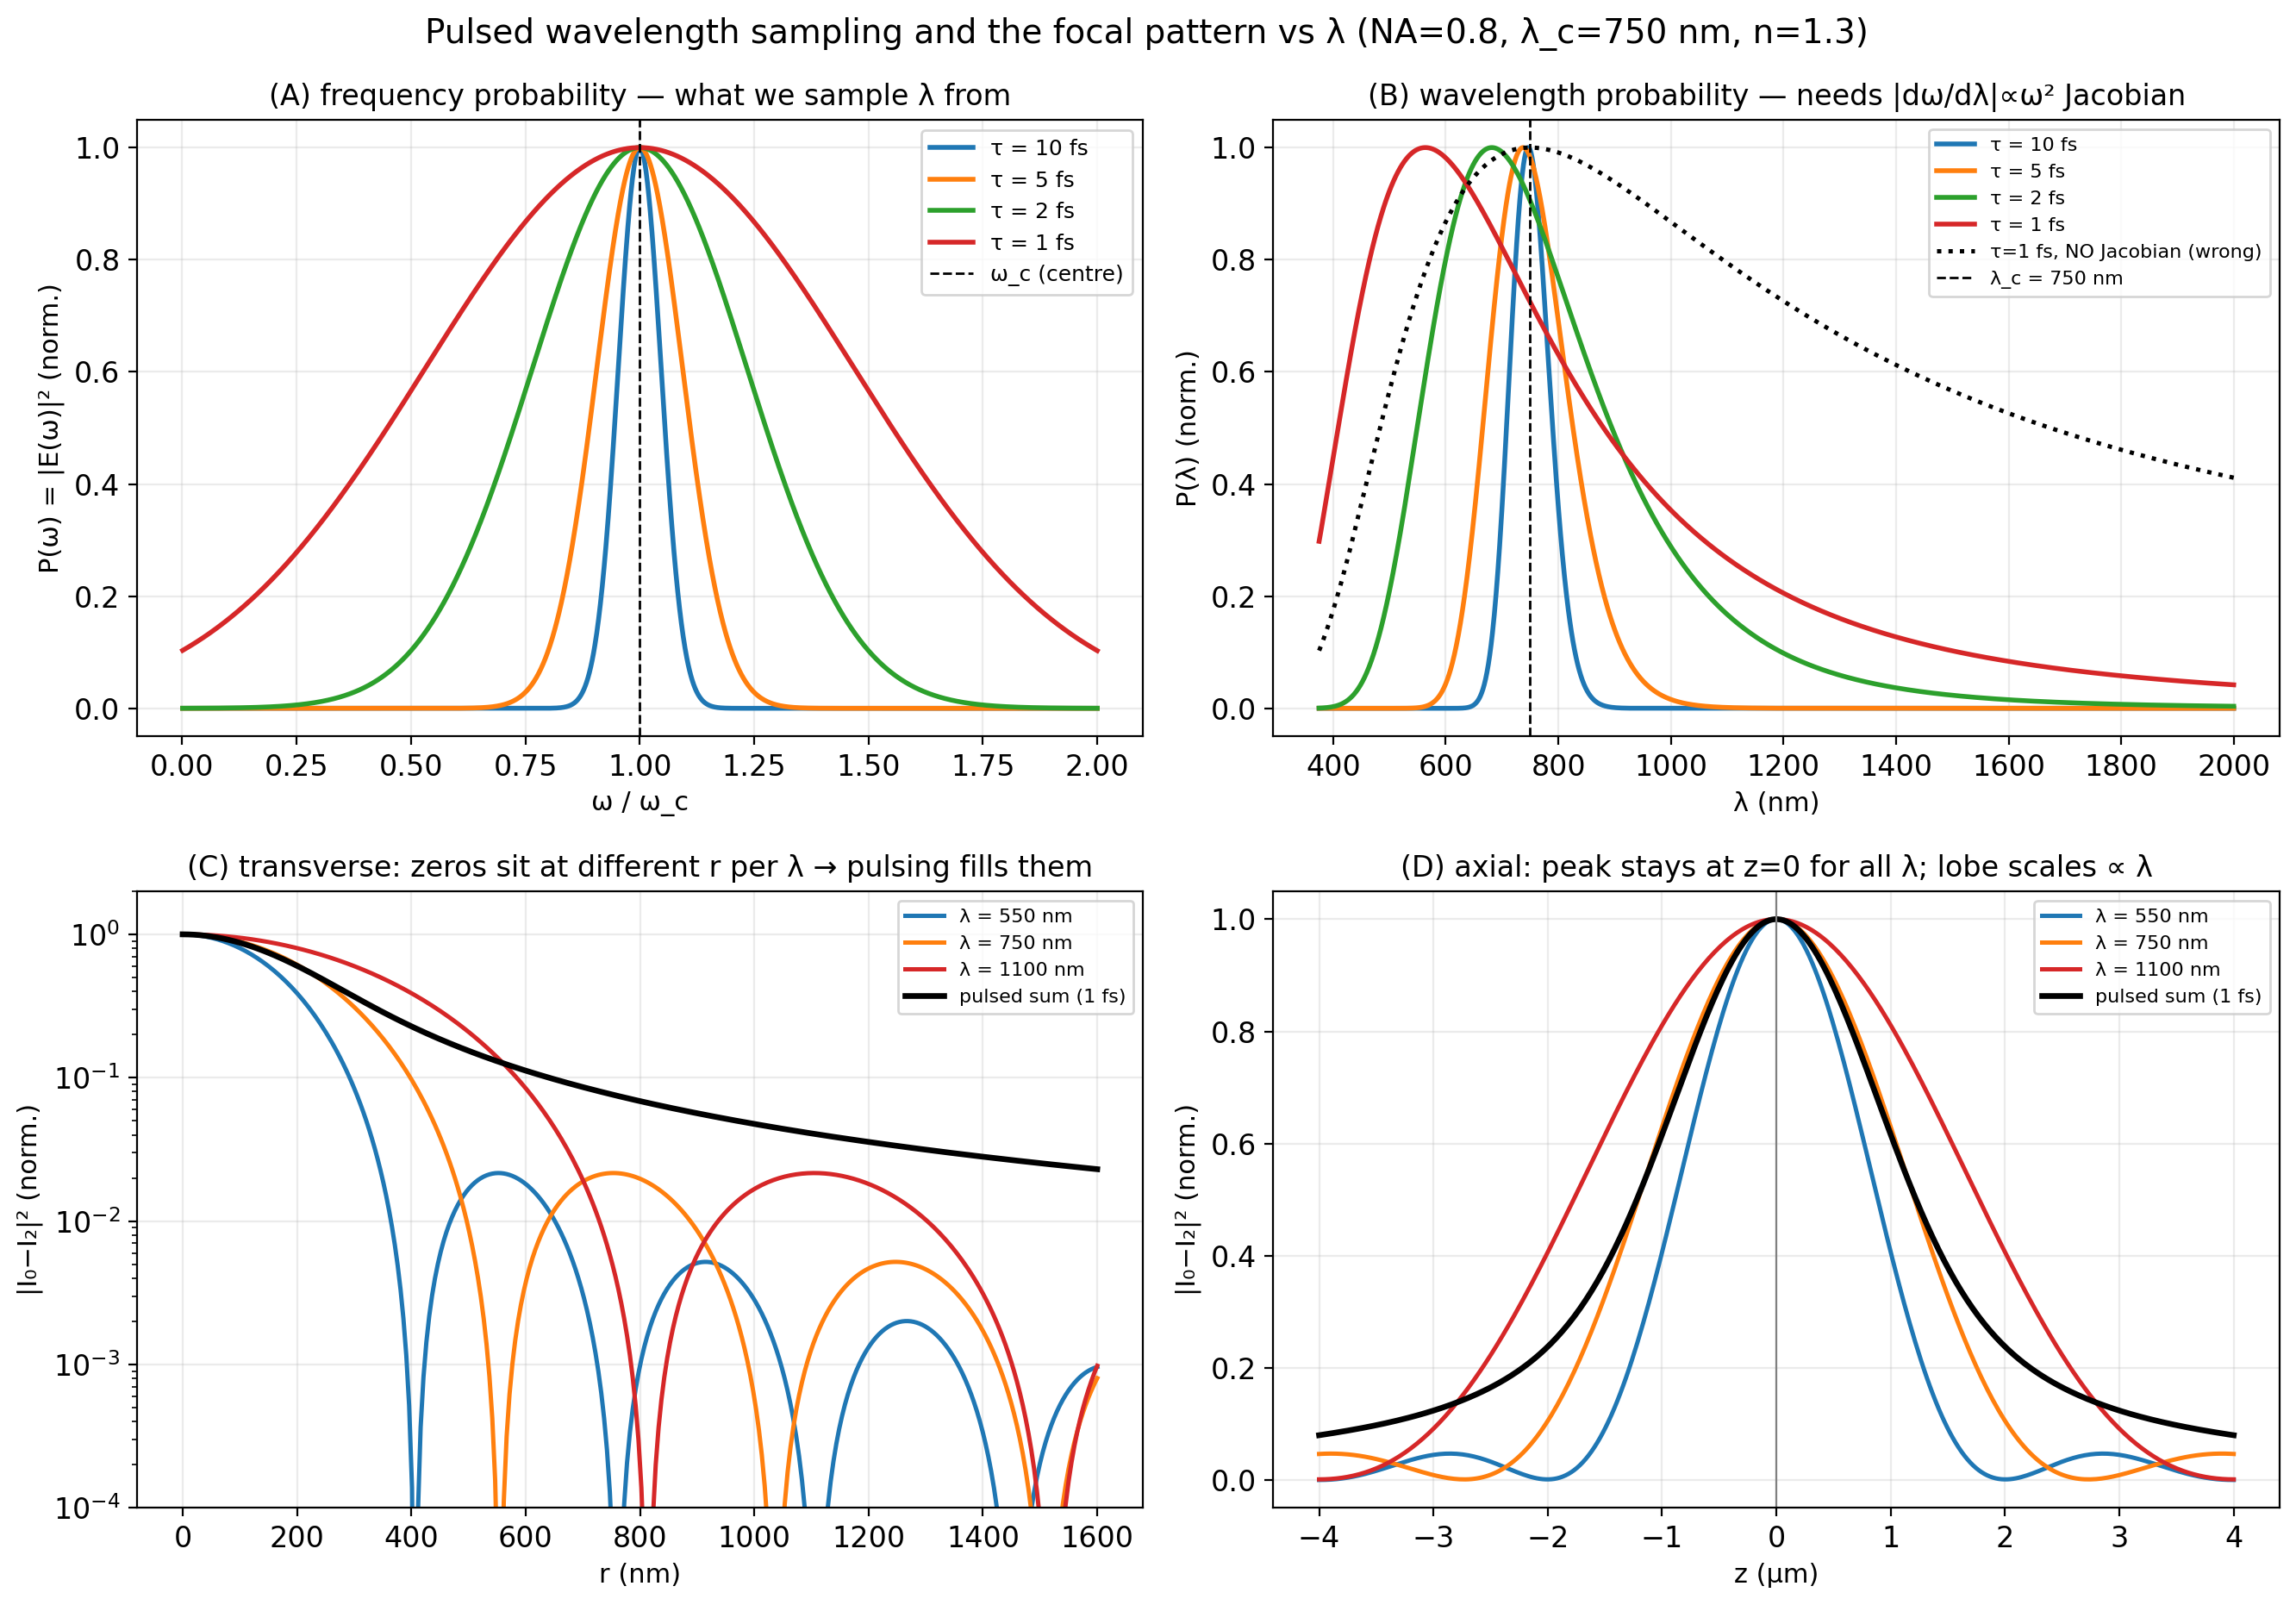
\includegraphics[width=0.99\textwidth]{spectral_sampling.png}\end{center}

\textbf{The $S(\tau)$ non-monotonicity is real}
(\texttt{pulsed\_S\_diagnostic.png}), not numerics or a single-cut artifact:
(A) the dip-then-rise is \emph{smooth} on a dense $\tau$ grid; (B) $S$ is
\emph{flat vs $N_{freq}$} (51--801) --- not spectral undersampling; (C) it appears
in the y-cut $|I_0-I_2|^2$, the x-cut $|I_0+I_2|^2+4|I_1|^2$, \emph{and} the full
azimuth-averaged $|I_0|^2+|I_2|^2+2|I_1|^2$ (all of $E_x,E_y,E_z$). Cross-check
$S$(5/2/1 fs)=0.988/0.987/1.057 reproduces the table above.
\begin{center}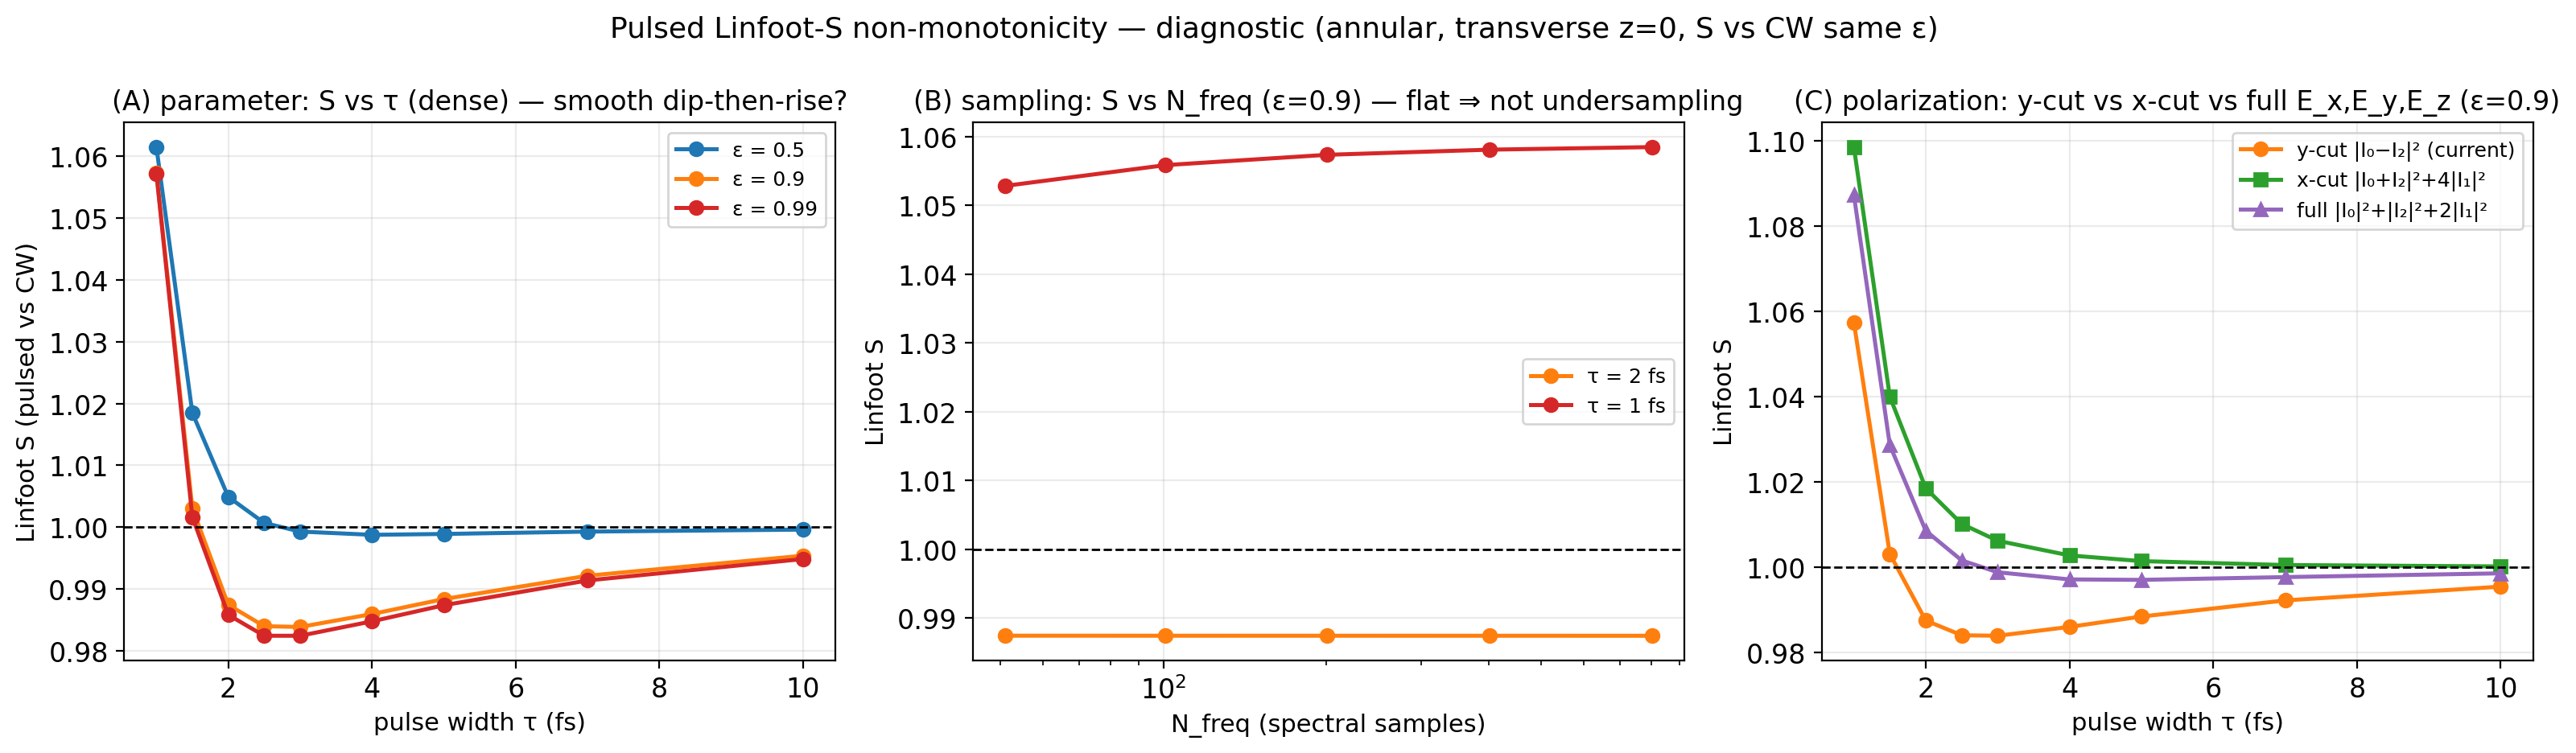
\includegraphics[width=0.99\textwidth]{pulsed_S_diagnostic.png}\end{center}
\end{document}
